\documentclass[tikz,border=0pt]{standalone}
\usepackage{amsmath}
\definecolor{bg}{HTML}{171D2B}
\definecolor{aksen}{HTML}{F7B538}
\definecolor{merah}{HTML}{E85D4A}
\definecolor{biru}{HTML}{6FB3D2}
\pagecolor{bg}
\begin{document}
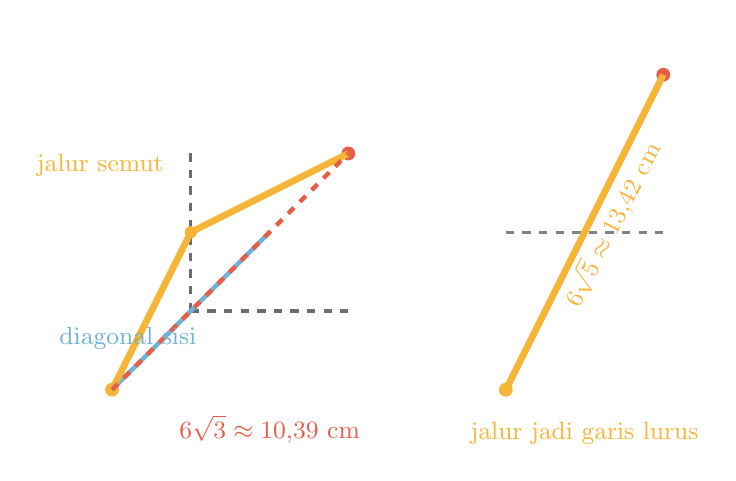
\begin{tikzpicture}[
  white, line width=1.1pt,
  label style/.style={font=\large\bfseries, text=white},
  semut/.style={color=aksen, line width=2.4pt},
  tembus/.style={dashed, color=merah, line width=1.6pt},
  sisi/.style={color=biru, line width=1.6pt}
]
% ---------- Kubus tertutup (kiri) ----------
\begin{scope}[shift={(0,0)}]
  \draw[white] (0,0) -- (2,0) -- (2,2) -- (0,2) -- cycle;          % sisi depan
  \draw[white] (1,1) -- (3,1) -- (3,3) -- (1,3) -- cycle;          % sisi belakang
  \draw[white] (0,2) -- (1,3);
  \draw[white] (2,2) -- (3,3);
  \draw[white] (2,0) -- (3,1);
  \draw[white] (1,3) -- (3,3);
  \draw[white] (3,1) -- (3,3);
  \draw[white] (1,3) -- (1,1);
  \draw[white] (1,1) -- (3,1);
  \draw[dashed, color=white!35!bg] (0,0) -- (1,1);
  \draw[dashed, color=white!35!bg] (1,1) -- (1,3);
  \draw[dashed, color=white!35!bg] (1,1) -- (3,1);
  \fill[aksen] (0,0) circle (2.5pt) node[label style, below left=1pt] {$A$};
  \fill[merah] (3,3) circle (2.5pt) node[label style, above right=1pt] {$C'$};
  % diagonal sisi depan (tetap di permukaan)
  \draw[sisi] (0,0) -- (2,2);
  % jalur semut lewat sisi depan + sisi atas, belok di rusuk (1,2)
  \draw[semut] (0,0) -- (1,2);
  \draw[semut] (1,2) -- (3,3);
  \fill[aksen] (1,2) circle (2.2pt);
  % diagonal ruang, menembus isi kubus
  \draw[tembus] (0,0) -- (3,3);
  \node[text=aksen, font=\small] at (-0.15,2.85) {jalur semut};
  \node[text=biru, font=\small] at (0.2,0.65) {\small diagonal sisi};
  \node[text=merah, font=\small] at (2.0,-0.5) {$6\sqrt{3}\approx 10{,}39$ cm};
\end{scope}

% ---------- Dua sisi dibentangkan (kanan) ----------
\begin{scope}[shift={(5.0,0)}]
  \draw[white] (0,0) -- (2,0) -- (2,2) -- (0,2) -- cycle;   % sisi depan
  \draw[white] (0,2) -- (2,2) -- (2,4) -- (0,4) -- cycle;   % sisi atas, dibuka
  \draw[dashed, color=white!45!bg] (0,2) -- (2,2);          % bekas rusuk lipatan
  \fill[aksen] (0,0) circle (2.5pt) node[label style, below left=1pt] {$A$};
  \fill[merah] (2,4) circle (2.5pt) node[label style, above=1pt] {$C'$};
  \draw[semut] (0,0) -- (2,4);
  \node[text=aksen, font=\small, rotate=63] at (1.35,2.1) {$6\sqrt{5}\approx 13{,}42$ cm};
  \node[text=aksen, font=\small] at (1.0,-0.55) {jalur jadi garis lurus};
\end{scope}
\end{tikzpicture}
\end{document}
